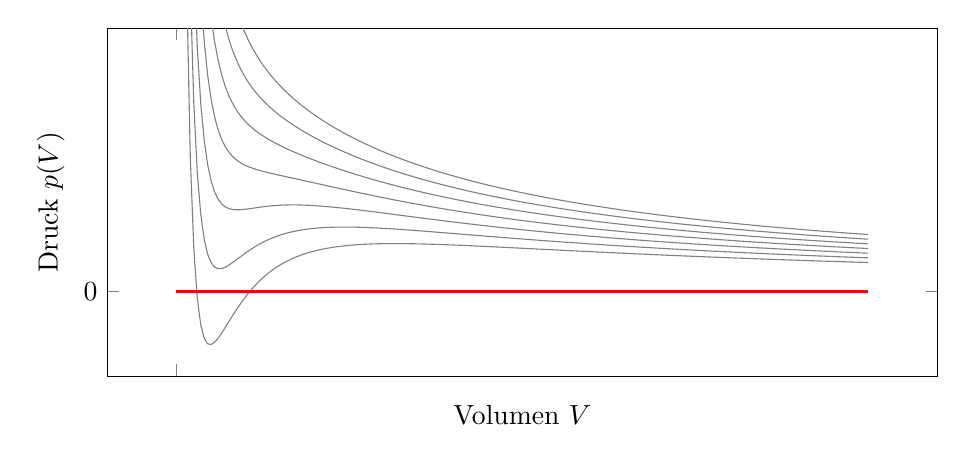
\begin{tikzpicture}
\pgfmathsetmacro{\a}{8000}
\pgfmathsetmacro{\b}{.9}
\pgfmathsetmacro{\R}{8.313}
\pgfmathsetmacro{\n}{1}
\pgfmathsetmacro{\T}{247}
\pgfmathsetmacro{\dT}{30}

\begin{axis}[
        width = \linewidth,
        height = 6cm,
        ylabel = Druck \(p(V)\),
        xlabel = Volumen \(V\),
        ytick = {0}, xtick = {1},
        yticklabels = {0},
        xticklabels = {},
        ymax = 1000,
        samples = 200,
        domain = 1:15, 
    ]

    \pgfplotsinvokeforeach{0,1,2,...,6}{
        \addplot[gray, variable=\V]
            {(\n*\R*(\T+#1*\dT))/(\V-\n*\b)-(\n^2*\a)/(\V^2)};
    }

    \addplot[thick,red]{0};
\end{axis}
\end{tikzpicture}
